\documentclass[aspectratio=169,10pt]{beamer}

% Shared Beamer setup for Fall 2026 course slides.
% Clean Cal Poly-inspired theme: no custom class files or uncommon packages.
\mode<presentation>{
  \usetheme{default}
  \usefonttheme{professionalfonts}
}

\definecolor{CalPolyGreen}{HTML}{154734}
\definecolor{CalPolyGold}{HTML}{BD8B13}
\definecolor{CalPolySage}{HTML}{7FA28F}
\definecolor{CalPolyMint}{HTML}{DDF1E7}
\definecolor{CalPolySand}{HTML}{A29F86}
\definecolor{CalPolyBeige}{HTML}{EFEEDE}
\definecolor{DeckInk}{HTML}{1F2933}
\definecolor{DeckMuted}{HTML}{5F6B7A}
\definecolor{DeckSoft}{HTML}{F7F7F5}

\setbeamersize{text margin left=0.55in,text margin right=0.55in}
\setbeamercolor{normal text}{fg=DeckInk,bg=white}
\setbeamercolor{structure}{fg=CalPolyGreen}
\setbeamercolor{title}{fg=white}
\setbeamercolor{frametitle}{fg=CalPolyGreen,bg=white}
\setbeamercolor{block title}{bg=CalPolySage,fg=white}
\setbeamercolor{block body}{bg=CalPolyMint,fg=black}
\setbeamercolor{alerted text}{fg=CalPolyGold}

\setbeamerfont{title}{size=\Huge,series=\bfseries}
\setbeamerfont{frametitle}{size=\Large,series=\bfseries}
\setbeamerfont{block title}{size=\normalsize,series=\bfseries}

\setbeamertemplate{navigation symbols}{}
\setbeamertemplate{itemize item}{\color{CalPolyGold}$\blacktriangleright$}
\setbeamertemplate{itemize subitem}{\color{CalPolyGreen}$\bullet$}
\setbeamertemplate{footline}{
  \hfill{\color{DeckMuted}\scriptsize\insertframenumber/\inserttotalframenumber}
  \hspace{0.18in}\vspace{0.12in}
}
\setbeamertemplate{frametitle}{
  \vspace{0.18in}
  \hspace{0.02in}\insertframetitle\par
  \vspace{0.08in}
  \noindent\makebox[\linewidth][l]{%
    {\color{CalPolyGold}\rule{0.55in}{2pt}}%
    {\color{CalPolyGreen}\rule{\dimexpr\linewidth-0.55in\relax}{2pt}}%
  }
}

\newcommand{\CourseNumber}{Course}
\newcommand{\CourseTitle}{Course Title}
\newcommand{\LectureNumber}{0}
\newcommand{\LectureTitle}{Lecture Title}
\newcommand{\LectureDate}{Date}
\newcommand{\CourseUnit}{Unit}

\newcommand{\coursenumber}[1]{\renewcommand{\CourseNumber}{#1}}
\newcommand{\coursetitle}[1]{\renewcommand{\CourseTitle}{#1}}
\newcommand{\lecturenumber}[1]{\renewcommand{\LectureNumber}{#1}}
\newcommand{\lecturetitle}[1]{\renewcommand{\LectureTitle}{#1}}
\newcommand{\lecturedate}[1]{\renewcommand{\LectureDate}{#1}}
\newcommand{\courseunit}[1]{\renewcommand{\CourseUnit}{#1}}

\author{Kirk Duran}
\institute{California Polytechnic State University, San Luis Obispo}
\date{\LectureDate}

\newcommand{\makedecktitle}{
  \begingroup
  \setbeamercolor{background canvas}{bg=CalPolyGreen}
  \begin{frame}[plain]
    \vfill
    \begin{center}
      {\usebeamerfont{title}\color{white}\LectureTitle\par}
      \vspace{0.18in}
      {\Large\color{white}Lecture \LectureNumber\par}
    \end{center}
    \vfill
    \noindent{\color{white}\rule{\linewidth}{1.2pt}}\par
    \vspace{0.08in}
    \noindent\colorbox{CalPolyGold}{\makebox[0.24\linewidth][c]{\color{white}\Large\CourseNumber}}
    \hspace{0.12in}{\color{white}\Large Kirk Duran}
  \end{frame}
  \endgroup
}

\newenvironment{keyidea}{\begin{block}{Key idea}}{\end{block}}
\newenvironment{activity}{\begin{block}{In class}}{\end{block}}
\newenvironment{cpdefinition}{\begin{block}{Definition}}{\end{block}}
\newenvironment{exampleblockcp}{
  \begingroup
  \setbeamercolor{block title}{bg=CalPolySand,fg=white}
  \setbeamercolor{block body}{bg=CalPolyBeige,fg=black}
  \begin{block}{Example}
}{
  \end{block}
  \endgroup
}

\newcommand{\imageplaceholder}[2][0.3in]{%
  \noindent\makebox[\linewidth][c]{%
    \fcolorbox{CalPolySage}{CalPolyBeige}{%
      \parbox[c][#1][c]{0.86\linewidth}{%
        \centering
        {\color{DeckMuted}\scriptsize Image placeholder: }%
        {\color{DeckInk}\scriptsize\ttfamily\detokenize{#2}}%
      }%
    }%
  }%
}

\newcommand{\sectionframe}[1]{
  \begingroup
  \setbeamercolor{background canvas}{bg=CalPolyGreen}
  \begin{frame}[plain]
    \vfill
    {\color{white}\LARGE\bfseries #1\par}
    \vspace{0.18in}
    {\color{CalPolyGold}\rule{0.22\paperwidth}{3pt}}
    {\color{white}\rule{0.62\paperwidth}{3pt}}
    \vfill
  \end{frame}
  \endgroup
}

\newcommand{\placeholdernote}{
  \begin{block}{Placeholder}
    Replace these bullets with the final lecture material, examples, and in-class activities.
  \end{block}
}


\usepackage{tikz}
\usetikzlibrary{arrows.meta,positioning,calc}

\graphicspath{{../assets/lecture-18/}}

% If an image file is not yet available, skip the visual slot.
\newcommand{\lectureimage}[2][1.75in]{%
  \IfFileExists{../assets/lecture-18/#2}{%
    \includegraphics[width=\linewidth,height=#1,keepaspectratio]{#2}%
  }{}%
}

% Explicit placeholder for visuals/examples that will be added later.
\newcommand{\lectureplaceholder}[2][2.35in]{%
  \begin{center}
    \fbox{%
      \begin{minipage}[c][#1][c]{0.90\linewidth}
        \centering
        \small\textit{#2}
      \end{minipage}%
    }
  \end{center}%
}

\setbeamersize{text margin left=0.42in,text margin right=0.42in}

\coursenumber{CS 4880}
\coursetitle{Artificial Intelligence}
\lecturenumber{18}
\lecturetitle{Probability and Bayesian Reasoning}
\lecturedate{October 7, 2026}
\courseunit{Probability and Bayesian Networks}

\begin{document}

% Estimated pacing: 50 minutes
% Motivation: 7 min
% Probability foundations and sensor model: 10 min
% Conditional probability and Bayes' rule: 15 min
% Multiple evidence, independence, and Naive Bayes: 13 min
% Engineering tradeoffs and transition: 5 min

% -----------------------------------------------------------------------------
% Slide 1
% -----------------------------------------------------------------------------
\makedecktitle

\section{A Route Is Not a World Model}

% -----------------------------------------------------------------------------
% Slide 2
% -----------------------------------------------------------------------------
\begin{frame}[shrink=10]{The Robot Already Knows How to Get There}
  \begin{columns}[T,onlytextwidth]
    \begin{column}{0.54\textwidth}
      A campus delivery robot has already computed a route with a path-finding algorithm.

      \begin{itemize}
        \item The map contains sidewalks, crossings, ramps, and buildings.
        \item The planner chooses a low-cost path to the destination.
        \item On the static map, the route is valid.
      \end{itemize}

      \begin{keyidea}
        Search can solve the route-planning problem perfectly relative to the map it was given.
      \end{keyidea}
    \end{column}
    \begin{column}{0.40\textwidth}
      \lectureimage[2.60in]{slide2.png}
    \end{column}
  \end{columns}
\end{frame}

% -----------------------------------------------------------------------------
% Slide 3
% -----------------------------------------------------------------------------
\begin{frame}[shrink=10]{But the Campus Is Not Static}
  \begin{columns}[T,onlytextwidth]
    \begin{column}{0.54\textwidth}
      Between planning and execution, the route may change:

      \begin{itemize}
        \item pedestrians stop in the walkway;
        \item bicycles cross the robot's path;
        \item maintenance carts appear;
        \item construction barriers move;
        \item temporary events block a sidewalk.
      \end{itemize}

      The map describes what \emph{should} be there. The robot must reason about what is there \emph{now}.
    \end{column}
    \begin{column}{0.40\textwidth}
      \lectureimage[2.65in]{slide3.png}
    \end{column}
  \end{columns}
\end{frame}

% -----------------------------------------------------------------------------
% Slide 4
% -----------------------------------------------------------------------------
\begin{frame}[shrink=10]{The Contingency Plan: Detect, Stop, Replan}
  A reasonable controller might contain a rule like:

  \[
    \text{if obstacle detected} \Rightarrow \text{stop and replan.}
  \]

  \begin{center}
    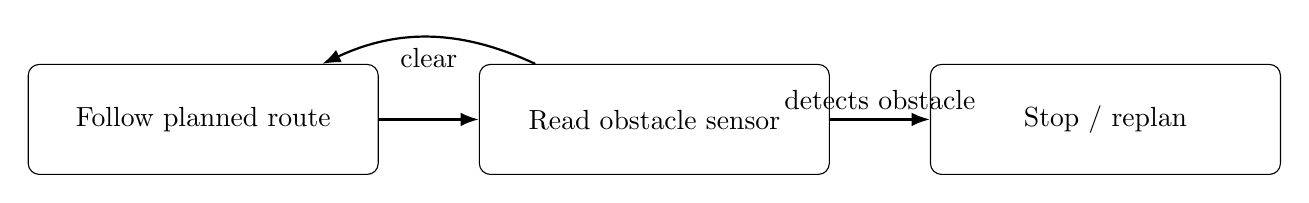
\begin{tikzpicture}[
      node distance=0.50in,
      every node/.style={draw,rounded corners,align=center,minimum width=1.75in,minimum height=0.55in},
      >=Latex
    ]
      \node (follow) {Follow planned route};
      \node (sense) [right=of follow] {Read obstacle sensor};
      \node (stop) [right=of sense] {Stop / replan};
      \draw[->,thick] (follow)--(sense);
      \draw[->,thick] (sense)--node[above,draw=none,minimum width=0in,minimum height=0in]{detects obstacle}(stop);
      \draw[->,thick,bend right=25] (sense) to node[below,draw=none,minimum width=0in,minimum height=0in]{clear}(follow);
    \end{tikzpicture}
  \end{center}

  \begin{keyidea}
    The planner is no longer the hard part. The hard part is deciding whether the sensor reading should be believed.
  \end{keyidea}
\end{frame}

% -----------------------------------------------------------------------------
% Slide 5
% -----------------------------------------------------------------------------
\begin{frame}[shrink=10]{Can the Sensor Ever Be Trusted 100\%?}
  \begin{columns}[T,onlytextwidth]
    \begin{column}{0.48\textwidth}
      Even a very good detector can produce:

      \begin{block}{False positive}
        The sensor reports an obstacle when the path is actually clear.
      \end{block}

      \begin{block}{False negative}
        The sensor reports clear when an obstacle is actually present.
      \end{block}
    \end{column}
    \begin{column}{0.46\textwidth}
      \lectureimage[2.55in]{slide5.png}
    \end{column}
  \end{columns}

  \begin{keyidea}
    Once perception can be wrong, the robot needs a language for uncertainty rather than only true/false rules.
  \end{keyidea}
\end{frame}

\section{Probability as a Model of Uncertainty}

% -----------------------------------------------------------------------------
% Slide 6
% -----------------------------------------------------------------------------
\begin{frame}[shrink=10]{Random Variables for the Robot}
  Define two binary random variables:

  \[
    O \in \{\text{obstacle},\;\neg\text{obstacle}\}
  \]

  \[
    S \in \{\text{sensor+},\;\text{sensor-}\}.
  \]

  We will abbreviate the events as
  \[
    O,\;\neg O,\;S,\;\neg S.
  \]

  \begin{cpdefinition}
    A random variable represents an uncertain quantity whose possible values are known even when its current value is not.
  \end{cpdefinition}

  \begin{keyidea}
    The obstacle either exists or does not. The uncertainty belongs to the robot's information state.
  \end{keyidea}
\end{frame}

% -----------------------------------------------------------------------------
% Slide 7
% -----------------------------------------------------------------------------
\begin{frame}[shrink=10]{A Probability Distribution Assigns Belief Mass}
  Suppose the robot's recent campus data suggests

  \[
    P(O)=0.10.
  \]

  Then, because $O$ is binary,

  \[
    P(\neg O)=1-P(O)=0.90.
  \]

  More generally, a valid distribution satisfies

  \[
    0\le P(x)\le 1
    \qquad\text{and}\qquad
    \sum_x P(x)=1.
  \]

  \begin{keyidea}
    Before the sensor reports anything, the robot already has a \textbf{prior} belief about how likely the path is to be blocked.
  \end{keyidea}
\end{frame}

% -----------------------------------------------------------------------------
% Slide 8
% -----------------------------------------------------------------------------
\begin{frame}[shrink=10]{The Prior Comes from Context}
  The value $P(O)=0.10$ is not a universal constant. It could depend on:

  \begin{itemize}
    \item time of day;
    \item location on campus;
    \item weather;
    \item class-change periods;
    \item construction schedules;
    \item the robot's recent observations.
  \end{itemize}

  \lectureimage[1.60in]{slide8.png}

  \begin{keyidea}
    Probability models encode assumptions about the environment. A wrong prior can distort even mathematically correct inference.
  \end{keyidea}
\end{frame}

% -----------------------------------------------------------------------------
% Slide 9
% -----------------------------------------------------------------------------
\begin{frame}[shrink=10]{The Sensor Model Is Conditional}
  Suppose calibration gives the detector the following behavior:

  \[
    P(S\mid O)=0.90
  \]

  \[
    P(S\mid \neg O)=0.05.
  \]

  Therefore

  \[
    P(\neg S\mid O)=0.10,
    \qquad
    P(\neg S\mid \neg O)=0.95.
  \]

  \begin{columns}[T,onlytextwidth]
    \begin{column}{0.47\textwidth}
      \begin{block}{Sensitivity / true-positive behavior}
        $P(S\mid O)$ asks how often the sensor fires when an obstacle really exists.
      \end{block}
    \end{column}
    \begin{column}{0.47\textwidth}
      \begin{block}{False-positive behavior}
        $P(S\mid \neg O)$ asks how often it fires on a clear path.
      \end{block}
    \end{column}
  \end{columns}
\end{frame}

% -----------------------------------------------------------------------------
% Slide 10
% -----------------------------------------------------------------------------
\begin{frame}[shrink=10]{From Conditionals to Joint Probabilities}
  The product rule gives

  \[
    P(A,B)=P(A)P(B\mid A).
  \]

  For the robot:

  \[
    P(O,S)=P(O)P(S\mid O)=0.10(0.90)=0.090
  \]

  \[
    P(O,\neg S)=0.10(0.10)=0.010
  \]

  \[
    P(\neg O,S)=0.90(0.05)=0.045
  \]

  \[
    P(\neg O,\neg S)=0.90(0.95)=0.855.
  \]

  \begin{keyidea}
    A joint probability refers to a complete combination of events: what the world is like \emph{and} what the sensor reports.
  \end{keyidea}
\end{frame}

% -----------------------------------------------------------------------------
% Slide 11
% -----------------------------------------------------------------------------
\begin{frame}[shrink=10]{How Often Does the Sensor Fire at All?}
  The sensor can fire in two mutually exclusive worlds:

  \begin{enumerate}
    \item an obstacle exists and the sensor fires;
    \item no obstacle exists and the sensor fires anyway.
  \end{enumerate}

  Therefore

  \[
    P(S)=P(O,S)+P(\neg O,S)
  \]

  \[
    P(S)=0.090+0.045=0.135.
  \]

  Likewise,

  \[
    P(\neg S)=0.010+0.855=0.865.
  \]

  \begin{keyidea}
    Marginalization sums over hidden alternatives that could have produced the observation.
  \end{keyidea}
\end{frame}

\section{Conditional Probability and Bayes' Rule}

% -----------------------------------------------------------------------------
% Slide 12
% -----------------------------------------------------------------------------
\begin{frame}[shrink=10]{The Direction We Know Is Not the Direction We Need}
  Calibration gave us

  \[
    P(S\mid O)=0.90.
  \]

  But after the robot observes a positive sensor reading, the operational question is

  \[
    \boxed{P(O\mid S)=?}
  \]

  These are not the same quantity.

  \begin{columns}[T,onlytextwidth]
    \begin{column}{0.47\textwidth}
      \begin{block}{$P(S\mid O)$}
        If there is an obstacle, how likely is the sensor to fire?
      \end{block}
    \end{column}
    \begin{column}{0.47\textwidth}
      \begin{block}{$P(O\mid S)$}
        If the sensor fired, how likely is there actually an obstacle?
      \end{block}
    \end{column}
  \end{columns}
\end{frame}

% -----------------------------------------------------------------------------
% Slide 13
% -----------------------------------------------------------------------------
\begin{frame}[shrink=10]{Conditional Probability Narrows the Sample Space}
  By definition,

  \[
    P(A\mid B)=\frac{P(A,B)}{P(B)}
  \]

  when $P(B)>0$.

  For our robot,

  \[
    P(O\mid S)=\frac{P(O,S)}{P(S)}.
  \]

  We already computed both terms:

  \[
    P(O,S)=0.090,
    \qquad
    P(S)=0.135.
  \]

  \begin{keyidea}
    Conditioning means restricting attention to the worlds consistent with the evidence and renormalizing their probability mass.
  \end{keyidea}
\end{frame}

% -----------------------------------------------------------------------------
% Slide 14
% -----------------------------------------------------------------------------
\begin{frame}[shrink=10]{Bayes' Rule Comes from the Product Rule}
  The same joint event can be written in two directions:

  \[
    P(A,B)=P(A)P(B\mid A)
  \]

  and

  \[
    P(A,B)=P(B)P(A\mid B).
  \]

  Set them equal:

  \[
    P(A)P(B\mid A)=P(B)P(A\mid B).
  \]

  Solve for $P(A\mid B)$:

  \[
    \boxed{P(A\mid B)=\frac{P(B\mid A)P(A)}{P(B)}}.
  \]

  \begin{keyidea}
    Bayes' rule reverses a conditional probability by combining a likelihood with a prior.
  \end{keyidea}
\end{frame}

% -----------------------------------------------------------------------------
% Slide 15
% -----------------------------------------------------------------------------
\begin{frame}[shrink=10]{Worked Example: Sensor Fires}
  We know

  \[
    P(O)=0.10,
    \qquad
    P(S\mid O)=0.90,
    \qquad
    P(S)=0.135.
  \]

  Apply Bayes' rule:

  \[
    P(O\mid S)
    =\frac{P(S\mid O)P(O)}{P(S)}
  \]

  \[
    =\frac{0.90(0.10)}{0.135}
    =\frac{0.090}{0.135}
    \approx \boxed{0.667}.
  \]

  \begin{keyidea}
    A positive sensor reading raises the obstacle probability from 10\% to about 67\%---strong evidence, but not certainty.
  \end{keyidea}
\end{frame}

% -----------------------------------------------------------------------------
% Slide 16
% -----------------------------------------------------------------------------
\begin{frame}[shrink=10]{Why Doesn't a 90\% Detector Give 90\% Confidence?}
  Among 1,000 comparable path segments, the model predicts approximately:

  \begin{center}
    \renewcommand{\arraystretch}{1.25}
    \begin{tabular}{l|r|r}
      & \textbf{Obstacle} & \textbf{Clear} \\\hline
      Sensor+ & 90 & 45 \\
      Sensor- & 10 & 855
    \end{tabular}
  \end{center}

  When the sensor fires, there are $90+45=135$ positive readings.

  Only 90 correspond to real obstacles:

  \[
    \frac{90}{135}=0.667.
  \]

  \begin{keyidea}
    The posterior depends on both sensor quality and the base rate of obstacles.
  \end{keyidea}
\end{frame}

% -----------------------------------------------------------------------------
% Slide 17
% -----------------------------------------------------------------------------
\begin{frame}[shrink=10]{Negative Evidence Also Updates Belief}
  Suppose the sensor reports clear. Then

  \[
    P(O\mid \neg S)
    =\frac{P(\neg S\mid O)P(O)}{P(\neg S)}.
  \]

  Substitute the model values:

  \[
    P(O\mid \neg S)
    =\frac{0.10(0.10)}{0.865}
    =\frac{0.010}{0.865}
    \approx \boxed{0.0116}.
  \]

  The robot's belief in an obstacle falls from 10\% to about 1.2\%.

  \begin{keyidea}
    Evidence can increase or decrease a belief; Bayesian updating is not inherently ``alarm seeking.''
  \end{keyidea}
\end{frame}

% -----------------------------------------------------------------------------
% Slide 18
% -----------------------------------------------------------------------------
\begin{frame}[shrink=10]{Probability Is Not Yet a Decision Rule}
  After a positive reading, we found

  \[
    P(O\mid S)\approx 0.667.
  \]

  Should the robot stop?

  \begin{itemize}
    \item Stopping unnecessarily costs time and battery.
    \item Continuing into a real obstacle can damage the robot or injure someone.
    \item Replanning may be cheap in one location and expensive in another.
  \end{itemize}

  \lectureimage[1.60in]{slide18.png}

  \begin{keyidea}
    Probability tells the agent what to believe. Choosing an action also requires costs, preferences, or utility---a later topic.
  \end{keyidea}
\end{frame}

\section{Multiple Evidence and Independence}

% -----------------------------------------------------------------------------
% Slide 19
% -----------------------------------------------------------------------------
\begin{frame}[shrink=10]{What If the Robot Samples Again?}
  Suppose the robot pauses briefly and obtains a second positive reading $S_2$ after the first $S_1$.

  We want

  \[
    P(O\mid S_1,S_2).
  \]

  A useful decomposition is

  \[
    P(O\mid S_1,S_2)
    \propto
    P(S_1,S_2\mid O)P(O).
  \]

  If the readings are conditionally independent given the true obstacle state,

  \[
    P(S_1,S_2\mid O)=P(S_1\mid O)P(S_2\mid O).
  \]

  \begin{keyidea}
    Multiple evidence can strengthen a belief, but only if we model how the evidence pieces relate to one another.
  \end{keyidea}
\end{frame}

% -----------------------------------------------------------------------------
% Slide 20
% -----------------------------------------------------------------------------
\begin{frame}[shrink=10]{Two Positive Readings: Update by Relative Weight}
  Under the conditional-independence assumption:

  \[
    w_O=P(O)P(S_1\mid O)P(S_2\mid O)
    =0.10(0.90)(0.90)=0.081
  \]

  \[
    w_{\neg O}=P(\neg O)P(S_1\mid \neg O)P(S_2\mid \neg O)
    =0.90(0.05)(0.05)=0.00225.
  \]

  Normalize:

  \[
    P(O\mid S_1,S_2)
    =\frac{0.081}{0.081+0.00225}
    \approx \boxed{0.973}.
  \]

  \begin{keyidea}
    Two apparently independent positive readings move the belief from 10\% prior to 67\% after one reading to about 97\% after two.
  \end{keyidea}
\end{frame}

% -----------------------------------------------------------------------------
% Slide 21
% -----------------------------------------------------------------------------
\begin{frame}[shrink=10]{But Are Two Readings Really Independent?}
  \begin{columns}[T,onlytextwidth]
    \begin{column}{0.53\textwidth}
      Repeated measurements from the same sensor may share the same failure cause:

      \begin{itemize}
        \item glare remains in the camera;
        \item a reflection persists across frames;
        \item a dirty lens affects every observation;
        \item the same occlusion hides the same obstacle;
        \item the same learned detector bias repeats.
      \end{itemize}
    \end{column}
    \begin{column}{0.41\textwidth}
      \lectureimage[2.55in]{slide21.png}
    \end{column}
  \end{columns}

  \begin{keyidea}
    Treating correlated evidence as independent can make the posterior dramatically overconfident.
  \end{keyidea}
\end{frame}

% -----------------------------------------------------------------------------
% Slide 22
% -----------------------------------------------------------------------------
\begin{frame}[shrink=10]{Independence Is a Modeling Claim}
  Two events $A$ and $B$ are independent when

  \[
    P(A,B)=P(A)P(B).
  \]

  Equivalently, when $P(B)>0$,

  \[
    P(A\mid B)=P(A).
  \]

  Conditional independence is different:

  \[
    P(A,B\mid C)=P(A\mid C)P(B\mid C).
  \]

  For repeated sensor readings we might assume

  \[
    S_1 \perp S_2 \mid O.
  \]

  \begin{keyidea}
    Independence is not something probability gives us for free. It is an assumption that simplifies the model.
  \end{keyidea}
\end{frame}

% -----------------------------------------------------------------------------
% Slide 23
% -----------------------------------------------------------------------------
\begin{frame}[shrink=10]{Normalization Turns Scores into Probabilities}
  Often we compute only proportional scores:

  \[
    P(O\mid e)\propto P(e\mid O)P(O).
  \]

  For binary $O$, define

  \[
    w_O=P(e\mid O)P(O),
    \qquad
    w_{\neg O}=P(e\mid \neg O)P(\neg O).
  \]

  Then

  \[
    P(O\mid e)=\frac{w_O}{w_O+w_{\neg O}}.
  \]

  Or write

  \[
    P(O\mid e)=\alpha P(e\mid O)P(O),
  \]

  where $\alpha$ is the normalizing constant that makes the probabilities sum to 1.
\end{frame}

% -----------------------------------------------------------------------------
% Slide 24
% -----------------------------------------------------------------------------
\begin{frame}[shrink=10]{Many Evidence Variables Become Expensive}
  Suppose the perception system produces evidence

  \[
    E_1,E_2,\ldots,E_n.
  \]

  In general, the robot would need

  \[
    P(E_1,E_2,\ldots,E_n\mid O),
  \]

  a joint model that accounts for every interaction among the evidence variables.

  \lectureimage[1.65in]{slide24.png}

  \begin{keyidea}
    Exact modeling becomes expensive because combinations of uncertain variables grow rapidly.
  \end{keyidea}
\end{frame}

\section{Naive Bayes}

% -----------------------------------------------------------------------------
% Slide 25
% -----------------------------------------------------------------------------
\begin{frame}[shrink=10]{Naive Bayes Makes a Deliberately Strong Assumption}
  Naive Bayes assumes that evidence variables are conditionally independent given the class:

  \[
    E_i \perp E_j \mid C.
  \]

  Then

  \[
    P(C\mid E_1,\ldots,E_n)
    \propto
    P(C)\prod_{i=1}^{n}P(E_i\mid C).
  \]

  For obstacle detection:

  \[
    P(O\mid E_1,\ldots,E_n)
    \propto
    P(O)\prod_iP(E_i\mid O).
  \]

  \begin{keyidea}
    The assumption is ``naive'' because the evidence is often not truly independent---but the simplification makes inference extremely cheap.
  \end{keyidea}
\end{frame}

% -----------------------------------------------------------------------------
% Slide 26
% -----------------------------------------------------------------------------
\begin{frame}[shrink=10]{Naive Bayes from One Sensor's Features}
  A single perception sensor can still produce several features:

  \begin{itemize}
    \item $E_1$: object-like shape detected;
    \item $E_2$: path region is visually occupied;
    \item $E_3$: detection persists across a short interval.
  \end{itemize}

  Suppose

  \[
    P(E_1\mid O)=0.85,\quad P(E_2\mid O)=0.80,\quad P(E_3\mid O)=0.75
  \]

  and

  \[
    P(E_1\mid \neg O)=0.08,\quad P(E_2\mid \neg O)=0.10,\quad P(E_3\mid \neg O)=0.15.
  \]

  \begin{keyidea}
    Naive Bayes converts a collection of simple feature likelihoods into a posterior over the class of interest.
  \end{keyidea}
\end{frame}

% -----------------------------------------------------------------------------
% Slide 27
% -----------------------------------------------------------------------------
\begin{frame}[shrink=10]{Worked Naive Bayes Classification}
  With prior $P(O)=0.10$:

  \[
    w_O=0.10(0.85)(0.80)(0.75)=0.051
  \]

  \[
    w_{\neg O}=0.90(0.08)(0.10)(0.15)=0.00108.
  \]

  Normalize:

  \[
    P(O\mid E_1,E_2,E_3)
    =\frac{0.051}{0.051+0.00108}
    \approx \boxed{0.979}.
  \]

  \begin{keyidea}
    The calculation is fast because we multiply small local likelihoods instead of storing one enormous joint distribution.
  \end{keyidea}
\end{frame}

% -----------------------------------------------------------------------------
% Slide 28
% -----------------------------------------------------------------------------
\begin{frame}[shrink=10]{The Engineering Tradeoff: Simplicity vs. Calibration}
  \begin{center}
    \renewcommand{\arraystretch}{1.35}
    \begin{tabular}{p{0.44\textwidth}|p{0.44\textwidth}}
      \textbf{What the simplifying assumptions buy us} & \textbf{What they can cost us} \\\hline
      compact probability tables & missed dependencies \\
      fast updates & overconfident posteriors \\
      easy estimation from data & sensitivity to biased training/calibration data \\
      interpretable likelihood terms & systematic errors may be counted repeatedly
    \end{tabular}
  \end{center}

  \begin{keyidea}
    A probability value can be numerically precise while the model that produced it is structurally wrong.
  \end{keyidea}
\end{frame}

\section{From One Sensor to Structured Uncertainty}

% -----------------------------------------------------------------------------
% Slide 29
% -----------------------------------------------------------------------------
\begin{frame}[shrink=10]{One Robot Quickly Becomes Many Random Variables}
  A realistic delivery robot may reason about

  \[
    \text{Pedestrian},\;\text{Bicycle},\;\text{Rain},\;\text{Visibility},\;\text{SensorReading},\;\text{BlockedPath},\ldots
  \]

  The challenge is no longer merely applying Bayes' rule once.

  We need to represent which variables directly influence which others so that we do \emph{not} store one full joint distribution over every combination.

  \lectureimage[2.00in]{slide29.png}

  \begin{keyidea}
    Next: Bayesian networks use graph structure to encode conditional independence and factor a large joint distribution.
  \end{keyidea}
\end{frame}

% -----------------------------------------------------------------------------
% Slide 30
% -----------------------------------------------------------------------------
\begin{frame}[shrink=10]{Takeaways}
  \begin{itemize}
    \item Random variables represent uncertain aspects of the world and the robot's observations.
    \item Priors encode what the agent believed before new evidence arrived.
    \item Conditional probabilities model sensor behavior under different world states.
    \item Bayes' rule converts likelihoods and priors into posterior beliefs.
    \item Multiple evidence can strengthen inference, but dependence matters.
    \item Normalization turns relative Bayesian scores into a valid probability distribution.
    \item Naive Bayes gains computational simplicity by assuming conditional independence.
    \item The recurring AI tradeoff is \textbf{model fidelity vs. computational tractability}.
  \end{itemize}

  \begin{keyidea}
    The robot should not ask ``Did the sensor say obstacle?'' It should ask ``Given what I knew before and what the sensor just reported, how strongly should I now believe an obstacle is present?''
  \end{keyidea}
\end{frame}

\end{document}
